\documentclass[letterpaper]{article}

\usepackage[letterpaper]{geometry}
\usepackage[log-declarations=false]{xparse}
\usepackage[quiet]{fontspec}
\usepackage{amsmath}
\usepackage{amsfonts}
\usepackage{enumerate}
\usepackage{polyglossia}
\usepackage{array}
\usepackage{graphicx}

\setdefaultlanguage{spanish}

\begin{document}
\title{Optimizacion No Lineal: Tarea 1}
\author{Ruben Astudillo \\ 201021009-k}
\date{\today}
\maketitle

\section*{Pregunta 1}
\noindent Para los ejemplos \(1\) y \(2\) de la ayudantia varie el
parametro \(\alpha\) y compare sus resultados. Para que valores de
\(\alpha\) no se tiene convergencia. Utilizar los metodos de maximo
descenso y de Newton.
\newline

Se analisaran individualmente cada una de las combinaciones. Para
desarrollar estos se realizaron en \texttt{octave} en vez de
\texttt{Matlab} por lo que pueden haber incompatibilidades que hayan
pasado por alto.󠀿

\subsection*{Ejemplo 1 con maximo descenso}
\noindent Nuestra funcion corresponde a
\[ f(x,y) = -10 + x^2 + y^2\]
\[ \nabla f (x,y) = [2 x , 2 y ] \]
Es claro que esta obtiene su minimo en \((0,0)\), por lo que podremos
comparar con respecto a este que tan lejos de la solucion termino el
algoritmo. El codigo se encuentra en la primera mitad del archivo
\texttt{pregunta\_1.m} donde se define \texttt{primer\_ej}
correspondiente a la funcion anterior. Dado que el punto inicial esta
dado en el ejemplo en \(x_0 = (1.5, 2.5)\) se respeta este valor como
partida, ademas utilizamos una toleracian de \(10e4\). A continuacion se
presenta los resultados de la computacion de \texttt{pregunta\_1.m} que
residen en \texttt{resultado\_1.txt} en formato de tabla
\[
\begin{array}{c c c}
  \alpha & \text{iteraciones} & \text{punto-final} \\
  \hline \\
  0.10 & 51    & (0.00, 0.00)   \\
  0.20 & 23    & (0.00, 0.00)   \\
  0.30 & 13    & (0.00, 0.00)   \\
  0.50 & 2     & (0.00, 0.00)   \\
  0.70 & 13    & (0.00, 0.00)   \\
  0.75 & 17    & (0.00, 0.00)   \\
  0.80 & 23    & (0.00, 0.00)   \\
  0.85 & 32    & (-0.00, -0.00) \\
  0.90 & 51    & (0.00, 0.00)   \\
  0.95 & 106   & (-0.00, -0.00) \\
  0.98 & 270   & (-0.00, -0.00) \\
  1.00 & 10000 & (-1.50, -2.50) \\
  1.20 & 2108  & (-\infty, NaN) \\
\end{array}
\]
Vemos que a medida que el \(\alpha\) tiende a \(1\) le cantidad de
iteraciones va llegando al maximo predefinido de iteraciones, despues de
este las soluciones se alejan del minimo \((0,0)\). Por tanto diremos que
para \(\alpha < 1\) el algoritmo de maximo descendo converge.

\subsection*{Ejemplo 1 con metodo de newton}
\noindent Similarmente que en la seccion anterior dados los mismos
parametros de inicio y toleracia junto con el hessiano de nuestra funcion
\[ H(x,y) =
  \begin{pmatrix}
    2 & 0 \\
    0 & 2
  \end{pmatrix}
  \qquad
  H^{-1}(x,y) =
  \begin{pmatrix}
    0.5 & 0 \\
    0 & 0.5
  \end{pmatrix}
\]
Se obtienen los siguientes resultados
\[
\begin{array}{c c c}
  \alpha & \text{iteraciones} & \text{punto-final} \\
  \hline \\
  1.00 & 2     & (0.00, 0.00)   \\
  1.20 & 8     & (-0.00, -0.00) \\
  1.40 & 13    & (0.00, 0.00)   \\
  1.60 & 23    & (0.00, 0.00)   \\
  1.80 & 51    & (0.00, 0.00)   \\
  1.90 & 106   & (-0.00, -0.00) \\
  1.95 & 215   & (0.00, 0.00)   \\
  1.99 & 1093  & (0.00, 0.00)   \\
  2.00 & 10000 & (-1.50, -2.50) \\
  2.10 & 7433  & (NaN, NaN)     \\
\end{array}
\]
Por lo que concluimos que para \(\alpha < 2\) hay convergencia.

\subsection*{Ejemplo 2 con maximo descenso}
\noindent Nuestra funcion cambia a
\[ f(x,y) = -10 + 3 x^2 + y^2 \]
\[ \nabla f (x,y) = [6 x , 2 y ] \]
Nuestras parametro siguen siendo iguales
\[
\begin{array}{c c c}
  \alpha & \text{iteraciones} & \text{punto-final} \\
  \hline \\
  0.20000 & 23    & (0.00, 0.00)  \\
  0.25000 & 18    & (-0.00, 0.00) \\
  0.30000 & 53    & (0.00, 0.00)  \\
  0.32000 & 138   & (-0.00, 0.00) \\
  0.33000 & 566   & (-0.00, 0.00) \\
  0.33333 & 10000 & (-1.50, 0.00) \\
  0.35000 & 7428  & (NaN, 0.00)   \\
\end{array}
\]
Por lo que concluimos que para \(\alpha < \frac 1 3 \) hay convergencia.

\subsection*{Ejemplo 2 con metodo de Newton}
\noindent Necesitamos calcular el hessiano de nuestra funcion
\[ H(x,y) =
  \begin{pmatrix}
    6 & 0 \\
    0 & 2
  \end{pmatrix}
  \qquad
  H^{-1}(x,y) =
  \begin{pmatrix}
    \frac{1}{6} & 0 \\
    0 & 0.5
  \end{pmatrix}
\]
\[
\begin{array}{c c c}
  \alpha & \text{iteraciones} & \text{punto-final} \\
  \hline \\
  1.40 & 14    & (-0.00, -0.00) \\
  1.60 & 24    & (-0.00, -0.00) \\
  1.80 & 53    & (0.00, 0.00)   \\
  1.90 & 111   & (0.00, 0.00)   \\
  1.95 & 227   & (0.00, 0.00)   \\
  1.98 & 573   & (0.00, 0.00)   \\
  1.99 & 1150  & (-0.00, -0.00) \\
  2.00 & 10000 & (-1.50, -2.50) \\
  2.10 & 7427  & (Inf, NaN)     \\
\end{array}
\]
por tanto se concluye que para \(\alpha < 2\) se converge.

\section*{Pregunta 2}
\noindent Minimice la funcion
\[ p(x,y) = \frac{1}{1 + (x-2)^2 + 2 (y+1)^2} + \frac{0.7}{1 + (x+1)^2 +
    2 (y - 2)^2 } \]
Utilizando el metodo de \emph{Leverberg-Marquardt}. Intente con distintos
valores de \(\alpha, \lambda\). Pruebe ademas con los valores iniciales
\((1.5, -2.5), (1.5, 2.5), (0,0), (1,1), (-3,-3)\). Compare los resultados.
\newline

Hemos de ver que en esta funcion, las variables solo ocurren dentro de
sub-expresiones cuadraticas, por lo tanto dado que los parametros son
positivos el valor minimo de \(p(x,y)\) es tendiente a \((0,0)\). El
grafico de la funcion podemos corroborar nuestra intuicion.
\begin{center}
  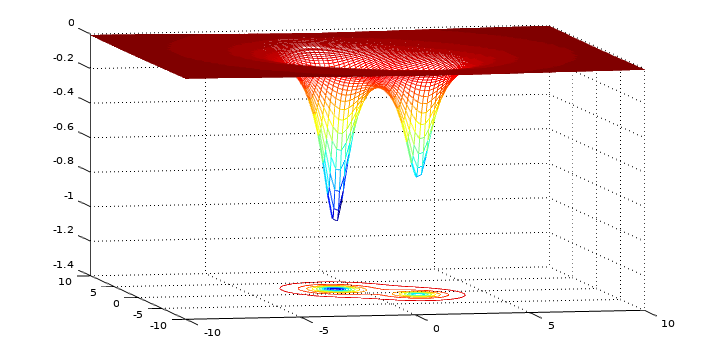
\includegraphics[scale=0.8]{pregunta2.png}
\end{center}
Por lo que nos da a pensar que el algoritmo va a alejarse de las
asimptotas. Para utilizar el algoritmo de \emph{Leverberg-Marquardt}
necesitamos conocer el gradiente y hessiano de \(p(x,y)\), las formulas
cerradas de estas funciones son largas, estan escrita de forma extendida
en el archivo \texttt{pregunta\_3.m} bajo el nombre de \texttt{fun\_grad}
y \texttt{fun\_hess} respectivamente. Nuestra estrategia para computar
aproximaciones en diferentes parametros se basa en iterar la rutina
\texttt{levenbert} sobre los puntos propuestos, sobre \(\lambda \in
[0.25, 1.6]\) y \(\alpha \in [0.25, 1.6]\), los cuales son valores que
muestran el algoritmo en su mejor forma. A continuacion solo dare un
esbozo de las computaciones que corresponden al primer parrafo en el
archivo de resultados \texttt{respuesta\_2.txt}.
\[
\begin{array}{c c c c c c}
  x_0 & \alpha & \lambda & \text{iteraciones} &
        (x_{\infty} = \text{punto-final}) & p(x_{\infty}) \\
  \hline \\
  (1.50, -2.50)  & 0.250 & 0.250 & 10000 & (1.06, -16.17)   & 0.00 \\
  (1.50, -2.50)  & 0.588 & 0.588 & 10000 & (1.01, -16.18)   & 0.00 \\
  (1.50, -2.50)  & 0.925 & 0.925 & 10000 & (1.00, -16.18)   & 0.00 \\
  (1.50, -2.50)  & 1.263 & 1.263 & 10000 & (0.99, -16.18)   & 0.00 \\
  (1.50, -2.50)  & 1.600 & 1.600 & 10000 & (0.99, -16.18)   & 0.00 \\
  (1.50, 2.50)   & 0.250 & 0.588 & 10000 & (5.45, 12.70)    & 0.01 \\
  (1.50, 2.50)   & 0.588 & 0.925 & 10000 & (5.77, 14.07)    & 0.00 \\
  (1.50, 2.50)   & 0.925 & 1.263 & 10000 & (5.90, 14.59)    & 0.00 \\
  (1.50, 2.50)   & 1.263 & 1.600 & 10000 & (5.96, 14.87)    & 0.00 \\
  (0.00, 0.00)   & 1.600 & 0.250 & 10000 & (-14.05, -22.28) & 0.00 \\
  (0.00, 0.00)   & 0.250 & 0.925 & 10000 & (-8.17, -8.29)   & 0.01 \\
  (0.00, 0.00)   & 0.588 & 1.263 & 10000 & (-9.08, -9.96)   & 0.01 \\
  (0.00, 0.00)   & 0.925 & 1.600 & 10000 & (-9.46, -10.70)  & 0.00 \\
  (1.00, 1.00)   & 1.263 & 0.250 & 10000 & (9.99, 23.22)    & 0.00 \\
  (1.00, 1.00)   & 1.600 & 0.588 & 10000 & (9.27, 19.74)    & 0.00 \\
  (1.00, 1.00)   & 0.250 & 1.263 & 10000 & (6.46, 9.66)     & 0.01 \\
  (1.00, 1.00)   & 0.588 & 1.600 & 10000 & (7.08, 11.50)    & 0.01 \\
  (-3.00, -3.00) & 0.925 & 0.250 & 10000 & (-10.19, -20.24) & 0.00 \\
  (-3.00, -3.00) & 1.263 & 0.588 & 10000 & (-9.38, -17.40)  & 0.00 \\
  (-3.00, -3.00) & 1.600 & 0.925 & 10000 & (-9.06, -16.37)  & 0.00 \\
  (-3.00, -3.00) & 0.250 & 1.600 & 10000 & (-6.01, -8.12)   & 0.01 \\
\end{array}
\]
Notemos que para distintos puntos iniciales, consistentemente llegamos al
tope de iteraciones. Al mismo tiempo siempre y cuando usemos \(\alpha < 1.6,
\lambda < 1.6\) nuestro punto final, si bien variado (dado el grafico de
la funcion) obtiene buenos minimos en la funcion objetivo.

\section*{Pregunta 3}
\noindent Minimice la funcion de \emph{Rosenbrock}
\[ f(x,y) = 100 (y - x^2)^2 + (1 - x)^2 \]
Utilizando los tres metodos vistos anteriormente y compare resultados
\newline

Los codigos estan en el archivo \texttt{pregunta\_3.m} con un ejemplo de
los resultados en \texttt{respuesta\_3.txt}. Es claro que el punto
minimizante de esta funcion corresponde a \((1,1)\), asi que tomamos solo
dos puntos iniciales, \(x_0 = (2.5, 3.5), x_0 = (-1,0) \) ambos no tan
lejos del minimo para analisar. Es bueno siempre tener la forma de la
funcion en mente
\begin{center}
  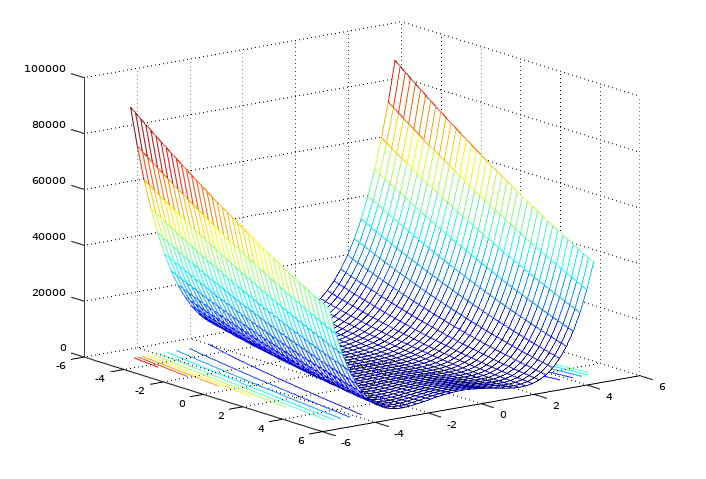
\includegraphics[scale=0.6]{pregunta3.png}
\end{center}

\subsection*{Maximo descenso}
Este corresponde a la primera seccion en el archivo
\texttt{respuesta\_3.txt}. Para utilizar este necesitamos el gradiente de
la funcion \(f\)
\[ \nabla f (x,y) = [-400 x (y - x^2) - 2 (1-x),\ 200 (y-x^2)] \]
Con esto, para \(x_0 = (2.5, 3.5)\) los resultados son los siguientes
\[
\begin{array}{c c c c c}
  x_0 & (x_{\infty} = \text{punto-final}) & \alpha & \text{iteraciones} &
    f(x_{\infty}) \\
  \hline \\
  (2.50, 3.50) & (1.79, 3.20)     & 0.0001 & 10000 & 0.62 \\
  (2.50, 3.50) & (1.61, 2.60)     & 0.0003 & 10000 & 0.37 \\
  (2.50, 3.50) & (1.44, 2.07)     & 0.0004 & 10000 & 0.19 \\
  (2.50, 3.50) & (1.28, 1.63)     & 0.0006 & 10000 & 0.08 \\
  (2.50, 3.50) & (1.14, 1.29)     & 0.0007 & 10000 & 0.02 \\
  (2.50, 3.50) & (1.02, 1.05)     & 0.0009 & 10000 & 0.00 \\
  (2.50, 3.50) & (0.99, 0.98)     & 0.0010 & 10000 & 0.00 \\
  (2.50, 3.50) & (1.01, 1.01)     & 0.0012 & 10000 & 0.00 \\
  (2.50, 3.50) & (NaN, \infty)    & 0.0013 & 11    & NaN  \\
  (2.50, 3.50) & (\infty, \infty) & 0.0015 & 10    & NaN  \\
\end{array}
\]
lo que nos dice que para este punto inicial, los valores de \(\alpha <
0.001\) hacen que el metodo converga eventualmente, a pesar de llegar a
nuestro limite (arbitrario) de iteraciones.

Para \(x_0 = (-1,0)\) hacemos el mismo procedimiento, obteniendo asi los
siguientes valores
\[
\begin{array}{c c c c c}
  x_0 & (x_{\infty} = \text{punto-final}) & \alpha & \text{iteraciones} &
    f(x_{\infty}) \\
  \hline \\
  (-1.00, 0.00) & (1.00, 1.00)      & 0.0020 & 9968  & 0.00 \\
  (-1.00, 0.00) & (0.88, 0.80)      & 0.0024 & 10000 & 0.14 \\
  (-1.00, 0.00) & (0.78, 0.66)      & 0.0028 & 10000 & 0.26 \\
  (-1.00, 0.00) & (0.71, 0.56)      & 0.0032 & 10000 & 0.37 \\
  (-1.00, 0.00) & (0.64, 0.47)      & 0.0036 & 10000 & 0.47 \\
  (-1.00, 0.00) & (0.65, 0.36)      & 0.0039 & 10000 & 0.51 \\
  (-1.00, 0.00) & (0.60, 0.30)      & 0.0043 & 10000 & 0.59 \\
  (-1.00, 0.00) & (0.56, 0.25)      & 0.0047 & 10000 & 0.66 \\
  (-1.00, 0.00) & (-\infty, \infty) & 0.0051 & 11    & NaN  \\
  (-1.00, 0.00) & (0.49, 0.16)      & 0.0055 & 10000 & 0.81 \\
\end{array}
\]
notar que tambien utiliza el maximo de iteraciones permitido, sin embargo
esta relativamente cerca de la solucion \((1,1)\), por lo que diremos que
para \(\alpha < 0.005\) el metodo de maximo descenso converge.

\subsection*{Metodo de Newton}
\noindent Corresponde a la segunda seccion del archivo
\texttt{respuesta\_3.txt}. Necesitamos el Hessiano de la funcion \(f\)
\[ H (x,y) =
  \begin{pmatrix}
    -400 y - 1200 x^2 + 2 & -400 x \\
    -400 x & 200
  \end{pmatrix}
\]
Notemos que para el valor \(x_0 = (2.5, 3.5)\) se tiene los siguientes resultados
\[
\begin{array}{c c c c c}
  x_0 & (x_{\infty} = \text{punto-final}) & \alpha & \text{iteraciones} &
    f(x_{\infty}) \\
  \hline \\
  (2.50, 3.50) & (3.48, 11.94)    & 0.0100 & 10000 & 8.38    \\
  (2.50, 3.50) & (0.86, 0.74)     & 0.0982 & 10000 & 0.03    \\
  (2.50, 3.50) & (1.04, 1.07)     & 0.1864 & 10000 & 0.00    \\
  (2.50, 3.50) & (1.22, 1.43)     & 0.2745 & 10000 & 0.30    \\
  (2.50, 3.50) & (1.18, 1.38)     & 0.3627 & 10000 & 0.04    \\
  (2.50, 3.50) & (0.95, 0.89)     & 0.4509 & 10000 & 0.01    \\
  (2.50, 3.50) & (2.26, 4.76)     & 0.5391 & 10000 & 12.68   \\
  (2.50, 3.50) & (50.59, 2558.77) & 0.6273 & 10000 & 2472.66 \\
  (2.50, 3.50) & (1.40, 1.75)     & 0.7155 & 10000 & 4.73    \\
  (2.50, 3.50) & (5.50, 30.03)    & 0.8036 & 10000 & 23.44   \\
  (2.50, 3.50) & (0.68, 0.43)     & 0.8918 & 10000 & 0.23    \\
  (2.50, 3.50) & (34.41, 1183.79) & 0.9800 & 10000 & 1148.27 \\
\end{array}
\]
notando que siempre llegamos al maximo de iteraciones para todos los
\(\alpha\), cuando \(\alpha > 0.92\) nos alejamos de la solucion
consistentemente y para valores \(\alpha < 0.42\) con nuestro tope de
iteraciones \(10000\) alcanzamos consistentemente la solucion.

Para \(x_0 = (-1,0)\) se obtiene por otra parte los siguientes resultados
\[
\begin{array}{c c c c c}
  x_0 & (x_{\infty} = \text{punto-final}) & \alpha & \text{iteraciones} &
    f(x_{\infty}) \\
  \hline \\
(-1.00, 0.00) & (1.00, 0.99)                    & 0.0100 & 10000 & 0.00   \\
(-1.00, 0.00) & (20.86, 435.14)                 & 0.1422 & 10000 & 395.88 \\
(-1.00, 0.00) & (1.05, 1.10)                    & 0.2744 & 10000 & 0.01   \\
(-1.00, 0.00) & (1.07, 1.14)                    & 0.4067 & 10000 & 0.00   \\
(-1.00, 0.00) & (1.12, 1.25)                    & 0.5389 & 10000 & 0.02   \\
(-1.00, 0.00) & (0.93, 0.84)                    & 0.6711 & 10000 & 0.05   \\
(-1.00, 0.00) & (-10.63, 112.92)                & 0.8033 & 10000 & 136.03 \\
(-1.00, 0.00) & (6.34, 39.69)                   & 0.9356 & 10000 & 60.90  \\
(-1.00, 0.00) & (-1074417.47, 1154372888868.30) & 1.0678 & 10000 & NaN \\
(-1.00, 0.00) & (24579.14, 604133898.00)        & 1.2000 & 10000 & NaN
\end{array}
\]
en todos los casos a costa de mas iteraciones podriamos tener mayor
precision pero con valores de \(\alpha < 0.75\) para nuestro tope de
iteraciones se obtienen buenas aproxiamaciones del valor \(x_1\), ademas
para valores de \(\alpha > 0.9\) consistentemente se diverge de la solucion.

En general este metodo tiene mejores propiedades de convergencia el de
maximo descenso para este problema. Tiene un rango de valores \(\alpha\)
mas amplio y mas estable que su alternativa.

\subsection*{Metodo de Levenberg}
La ultima seccion del archivo. Este metodo para todos los valores de
\(\alpha \in [0.1,\ 1.3]\) y \(\lambda \in [0.1,\ 1.3]\) probados
converge al valor \((1,1)\) dicho anteriormente. Solo mostraremos una
pequeña seccion de esta computacion pues todos los resultados son muy
homogeneos para ambos valores de \(x_0 = (2.5, 3.5), x_0 = (-1,0)\)

\[ \begin{matrix}
    x_{0} & x_{\infty} & \lambda & \alpha & \text{iteraciones} & f(x_{\infty}) \\
  \end{matrix}
\]
\[
\begin{tabular}{c c c c c c}
  \hline \\
(2.50, 3.50)  & (1.00, 1.00) & 0.10 & 0.10 & 202 & 0.00 \\
(2.50, 3.50)  & (1.00, 1.00) & 0.37 & 0.10 & 261 & 0.00 \\
(2.50, 3.50)  & (1.00, 1.00) & 0.50 & 0.37 & 82  & 0.00 \\
(2.50, 3.50)  & (1.00, 1.00) & 0.63 & 0.63 & 52  & 0.00 \\
(2.50, 3.50)  & (1.00, 1.00) & 0.77 & 0.90 & 40  & 0.00 \\
(2.50, 3.50)  & (1.00, 1.00) & 0.90 & 1.17 & 35  & 0.00 \\
(2.50, 3.50)  & (1.00, 1.00) & 1.17 & 0.10 & 491 & 0.00 \\
(2.50, 3.50)  & (1.00, 1.00) & 1.30 & 0.37 & 143 & 0.00 \\
(-1.00, 0.00) & (1.00, 1.00) & 0.10 & 0.63 & 35  & 0.00 \\
(-1.00, 0.00) & (1.00, 1.00) & 0.23 & 0.90 & 25  & 0.00 \\
(-1.00, 0.00) & (1.00, 1.00) & 0.37 & 1.17 & 27  & 0.00 \\
(-1.00, 0.00) & (1.00, 1.00) & 0.63 & 0.10 & 294 & 0.00 \\
(-1.00, 0.00) & (1.00, 1.00) & 0.77 & 0.37 & 91  & 0.00 \\
(-1.00, 0.00) & (1.00, 1.00) & 0.90 & 0.63 & 57  & 0.00 \\
(-1.00, 0.00) & (1.00, 1.00) & 1.03 & 0.90 & 42  & 0.00 \\
(-1.00, 0.00) & (1.00, 1.00) & 1.17 & 1.17 & 33  & 0.00 \\
\end{tabular}
\]
Algo interesante a considerar es la consistencia de la cantidad de
iteraciones que le toma llegar al optimo, siempre tomando a lo mas 300
iteraciones y siempre llegando al punto minimo de la funcion. Podemos
considerar que con mayor certeza este metodo para el cual este problema
converge.
\end{document}
